\documentclass[conference]{IEEEtran}
\usepackage{cite}
\usepackage{graphicx}
\usepackage{placeins}
\usepackage{textcomp}
\usepackage{caption}
\usepackage{tabto}
\usepackage{subfigure}
\usepackage{enumerate}
\usepackage{afterpage}
\usepackage{subfig}
\usepackage{subcaption} 
\usepackage[font={small}]{caption}
\AtBeginDocument{\renewcommand{\abstractname}{Resumo}}
\begin{document}
\title{Projeto 4 de Princ\'ipios de Vis\~ao Computacional}
\author{\IEEEauthorblockN{Gabriel Martins de Miranda}
\IEEEauthorblockA{130111350\\
Universidade de Bras\'ilia\\
Email:gabrielmirandat@hotmail.com}
}
\maketitle
\begin{abstract}
A presente demonstra\c{c}\~ao faz uso do programa $Find$-$Object$ criado por Mathieu Labbé. Nele \'e poss\'ivel 
combinar v\'arios detectores e descritores usados para reconhecer e acompanhar um objeto numa cena. Os objetos usados para as
compara\c{c}\~oes entre os diferentes m\'etodos foram $uma $ $dama $ $da $ $carta $ $de $ $baralho$ e 
$um $ $controle $ $remoto $ $para $ $DVD $ $player$. Os detectores/descritores usados foram: $SIFT$/$SIFT$ , $SURF$/$SURF$ , 
$FAST$/$BRIEF$ e $ORB$/$ORB$.


\end{abstract}

\section{ Introdu\c{c}\~ao} 
\label{sec:meth} 
	 \nobreak\hspace{.16667em plus .08333em} 
	 A primeira coisa que tem-se que ter em mente \'e a diferen\c{c}a entre os termos $detector$ e $descritor$. 
	 $detector$ se refere ao m\'etodo usado para se detectar as features.				    
	 $descritor$ se refere ao m\'etodo usado para casar as features encontradas de uma imagem em outra.
	 
	 Vamos introduzir agora uma breve explica\c{c}\~ao dos m\'etodos utilizados: \\
	 
	 1) $SIFT$/$SIFT$	\\
	 $SIFT$ - Scale-Invariant Feature Transform \\
	 Sift \'e um detector e descritor. Ele usa a invari\^ancia \`a rota\c{c}\~ao do 
	 detector de cantos de Harris e corrige a n\~ao-invari\^ancia \`a escala utilizando diferen\c{c}a da gaussiana (DoG) para
	 v\'arios tamanhos de escala. Ap\'os isto, os keypoints encontrados s\~ao refinados e s\~ao
	 eliminados qualquer keypoint de baixo contraste e de borda, e o que sobra s\~ao pontos de interesse mais robustos.
	 Logo em seguida, uma orienta\c{c}\~ao \'e atribu\'ida a cada keypoint para que se conquiste invari\^ancia \`a rota\c{c}\~ao
	 na imagem. Uma vizinhan\c{c}a dependente de escala, al\'em da magnitude do gradiente e dire\c{c}\~ao s\~ao calculados
	 na regi\~ao. Um histograma de orienta\c{c}\~oes com peso \'e criado. Ao final desta etapa s\~ao criados keypoints 
	 com mesma localiza\c{c}\~ao e escala, mas dire\c{c}\~oes diferentes. Isto contribui para a estabilidade do matching.
	 Para o descritor do keypoint, uma vizinha\c{c}a 16x16 \'e tomada e divida em 16 sub-blocos 4x4. Para cada sub-bloco, 
	 8 orienta\c{c}\~oes de histograma s\~ao criados. Logo, temos um total de 128 valores de histograma dispon\'iveis.
	 Isto \'e representado por um vetor para formar o descritor do keypoint. Em adi\c{c}\~ao a isto, v\'arias medidas s\~ao
	 tomadas para se obter robustez contra mudan\c{c}as de ilumina\c{c}\~ao, rota\c{c}\~ao, etc.
	 Ao final, os keypoints entre duas imagens s\~ao casados identificando-se seus vizinhos mais pr\'oximos. Por\'em, pode
	 ocorrer de o segundo casamento mais pr\'oximo para um mesmo ponto ser bem pr\'oximo do primeiro. Neste caso, a
	 rela\c{c}\~ao entre os dois \'e tomada, e se for maior que $0,8$, s\~ao ambos rejeitados. Isto elimina perto de 90\%
	 de falsos matches enquanto descarta apenas 5\% de matches corretos.
	 Devido \`a grande quantidade de c\'alculos utilizados, SIFT \'e considerado devagar em rela\c{c}\~ao aos m\'etodos 
	 que se seguem. \\
	 
	 2) $SURF$/$SURF$			\\
	 $SURF$ - Speeded-Up Robust Features	\\
	 Como o nome sugere, \'e uma vers\~ao acelerada do SIFT. No SIFT, Lowe aproximou o laplaciano da gaussiana (LoG) pela 
	 diferen\c{c}a da gaussiana (DoG) para encontrar invari\^ancia escala-espa\c{c}o. SURF aproxima o Log com filtro de 
	 caixa. A convolu\c{c}\~ao com o filtro de caixa pode ser facilmente calculada com a ajuda de imagens integrais. E isto
	 pode ser feito paralelamente para diferentes escalas. SURF tamb\'em depende do determinante da matriz Hessiana para 
	 invari\^ancia \'a escala e localiza\c{c}\~ao.
	 Para assinalar orienta\c{c}\~ao, SURF usa respostas wavelet nas dire\c{c}\~oes horizontal e vertical para uma 
	 vizinhan\c{c}a de tamanho 6. Pesos gaussianos adequados tamb\'em s\~ao aplicados. A orienta\c{c}\~ao dominante \'e 
	 estimada calculando-se a soma de todas as respostas dentro de uma janela de orienta\c{c}\~ao deslizante de 60\textdegree. Para 
	 v\'arias aplica\c{c}\~oes, a invari\^ancia \`a rota\c{c}\~ao n\~ao \'e necess\'aria, ent\~ao n\~ao se precisa achar 
	 esta orienta\c{c}\~ao, o que torna o processo mais r\'apido.
	 Para o descritor, SURF usa resposta wavelet nas dire\c{c}\~oes horizontal e vertical (novamente, o uso da imagem integral 
	 faz as coisas ficarem mais f\'aceis). Uma vizinhan\c{c}a de tamanho 20 \'e tomada em volta do keypoint. Ela \'e divida 
	 em sub-regi\~oes 4x4. Para cada sub-regi\~ao, respostas wavelet vertical e horizontal s\~ao tomadas e um vetor \'e 
	 formado, de dimens\~ao 64. Quanto menor a dimens\~ao, maior a velocidade dos c\'alculos e matching, por\'em diminui 
	 a distin\c{c}\~ao das features.
	 
	 H\'a uma vers\~ao de dimens\~ao 128, mais robusta, que n\~ao adiciona tanta complexidade computacional. Outra melhora 
	 importante \'e o uso do sinal do laplaciano (tra\c{c}o da matriz hessiana) para destacar o ponto de interesse. N\~ao
	 adiciona custo pois j\'a \'e calculado na detec\c{c}\~ao. Ela distingue bolhas claras em fundos escuros da situa\c{c}\~ao
	 inversa. No est\'agio de matching, apenas comparamos features se tiverem o mesmo tipo de contraste. Isto permite velocidade 
	 sem reduzir a performance do descritor. An\'alises indicam que o SURF \'e tr\^es vezes mais r\'apido comparado ao 
	 SIFT enquanto que possui performance similar.
	 
	 SURF \'e bom manipulando imagens com borrado e rota\c{c}\~ao, mas n\~ao bom com mudan\c{c}as no ponto de vista e de 
	 ilumina\c{c}\~ao. \\
	 
	 3)$FAST$/$BRIEF$					\\
	 $FAST$ - Features from Accelerated Segment Test	\\
	 \'E importante destacar que FAST \'e um algoritmo  apenas de detec\c{c}\~ao, usado para detec\c{c}\~ao de cantos.
	 Vimos muitos detectores de features, mas para aplica\c{c}\~oes em tempo real, eles n\~ao s\~ao r\'apidos o bastante.
	 Um exemplo da necessidade de velocidade \'e em SLAM mobile robot, que tem recursos computacionais limitados. Os passos
	 utilizados pelo algoritmo s\~ao:	\\
	    a) Encontrar um ponto p de intensidade Ip.	\\
	    b) Escolher um limiar t.	\\
	    c) Fazer um c\'irculo de 16 pixels em volta do pixel p. \\
	    p ser\'a canto se existem n pixels do c\'irculo cont\'iguo mais claros que Ip + t ou mais escuros que Ip - t.
	    \\ n por padr\~ao foi escolhido como 12.	\\
	    d) Teste para excluir grande n\'umero de n\~ao-cantos. Um grande problema do teste \'e que v\'arias features s\~ao 
	    detectadas umas adjacentes \`as outras. Dos 4 pontos considerados no teste, os 3 primeiros s\~ao endere\c{c}ados 
	    com uma abordagem de aprendizado de m\'aquina enquanto o \'ultimo usa supress\~ao de n\~ao-m\'aximos.	\\
	    
	    Estudos indicam que FAST \'e diversas vezes mais r\'apido que qualquer outro detector de bordas.	\\
	    
	  $BRIEF$ - Binary Robust Independent Elementary Features						\\
	  \nobreak\hspace{.16667em plus .08333em} 
	  Aqui novamente deve-se dizer que BRIEF \'e um m\'etodo descritor, e n\~ao detector.
	  SIFT usa vetores para descritores de tamanho 128, o que toma basicamente 512 bytes de mem\'oria por vetor. SURF similarmente 
	  usa um de 64, com m\'inimo de 256 bytes. Criar um vetor assim para milhares de features toma um monte de mem\'oria 
	  que n\~ao \'e vi\'avel com recursos limitados e sistemas embarcados. Quanto maior a mem\'oria, maior o tempo gasto 
	  para matching.
	  Toda esta dimens\~ao pode ser comprimida usando v\'arios m\'etodos, como PCA, LDA, etc. Um deles, o LSH (Locality 
	  Sensitive Hashing) \'e usado para converter estes descritores SIFT de floats para n\'umeros bin\'arios usando 
	  hashing. Essas strings bin\'arias s\~ao usadas para casar features usando dist\^ancia de Hamming. Isso d\'a muita 
	  velocidade pois para encontrar a dist\^ancia de Hamming \'e s\'o aplicar uma XOR e contagem de bits, coisas r\'apida nas 
	  CPUs modernas. 
	  Por\'em, primeiro precisamos encontrar os descritores, s\'o assim podemos aplicar hashing , o que n\~ao soluciona 
	  o problema de mem\'oria. BRIEF chega neste momento.
	  Ele nos d\'a um atalho para encontrar as strings bin\'arias diretamente sem encontrar os descritores.
	  Ele toma peda\c{c}os da imagem borrados e seleciona um set de pares localizados. Da\'i algumas compara\c{c}\~oes de 
	  intensidade de pixels s\~ao feitas nestes pares. Assim s\~ao constru\'idas as strings de bits. Por padr\~ao este 
	  vetor possui tamanho 256 e \'e representado por 32 bytes. Ent\~ao, a partir dele, voc\^e pode calcular a dist\^ancia 
	  de Hamming para casar estes descritores. 
	  Como foi dito anteriormente, BRIEF \'e um feature descriptor, ele n\~ao prov\^e m\'etodos para encontrar features.
	  Logo, deve-se usar qualquer outro feature detector, como SIFT, SURF, etc. O paper recomenda usar o detector CenSurE
	  (conhecido como STAR  no OpenCV), que casa melhor com o BRIEF que o SIFT.
	  BRIEF \'e o mais r\'apido descritor, prov\^e alto grau de matching desde que n\~ao haja grandes rota\c{c}\~oes no
	  plano.	\\
	  
	  4)$ORB$/$ORB$					\\
	 $ORB$ - Oriented FAST and rotated BRIEF	\\
	 Criado no OpenCV Labs. \'E uma alternativa ao SIFT e ao SURF em termos de custo computacional, performance 
	 de matching e principalmente as patentes. (Ele \'e free, ao contr\'ario dos outros dois).
	 ORB \'e basicamente uma fus\~ao do detector FAST com o descritor BRIEF com v\'arias modifica\c{c}\~oes para melhorar 
	 a performance. 
	 Primeiro se usa o FAST para encontrar keypoints, depois Harris para encontrar os top N pontos entre eles. Tamb\'em 
	 usa pir\^amide para encontrar features- multiescalados. O problema \'e que FAST n\~ao calcula as orienta\c{c}\~oes, 
	 o que n\~ao \'e invariante \'a rota\c{c}\~ao. Ent\~ao os autores modificaram para obter esta caracter\'istica.
	 Isto calcula a intensidade ponderada do centroid do peda\c{c}o cujo canto est\'a localizado no centro. A dire\c{c}\~ao 
	 do vetor que vai do canto at\'e o centroid nos d\'a a orienta\c{c}\~ao. A inveri\^ancia \`a rota\c{c}\~ao tamb\'em 
	 \'e melhorada.
	 Para os descritores, ORB usa o descritor BRIEF. Mas j\'a vimos que o BRIEF \'e pobre com rota\c{c}\~ao. ORB ent\~ao 
	 "direciona" BRIEF de acordo com a orienta\c{c}\~ao dos keypoints. ORB contr\'oi uma look up table de padr\~oes pr\'e-
	 computados do BRIEF. Contando que a orienta\c{c}\~ao do keypoint seja consistente, o set correto de pontos do BRIEF 
	 com rota\c{c}\~ao \'e usado para computar o descritor.
	 BRIEF tem uma caracter\'istica importante que cada feature do bit tem larga vari\^ancia e m\'edia perto de 0.5. Por\'em, 
	 uma vez que est\'a orientado com a dire\c{c}\~ao do keypoint, ele perde essa propriedade e se torna mais distribu\'ido. 
	 Grande vari\^ancia faz uma feature mais discriminativa, desde que responde diferentemente \`as entradas. Outra
	 propriedade desejada \'e ter os testes n\~ao correlacionados, j\'a que cada teste vai contribuir para o resultado.
	 Para resolver isto, ORB procura entre todas as possibilidades de testes bin\'arios para encontrar aqueles que tem 
	 tanto grande vari\^ancia e m\'edia perto de 0.5, assim como n\~ao sendo correlacionados. O resultado \'e chamado 
	 rBRIEF.
	 O paper diz que ORB \'e bem mais r\'apido que SURF e SIFT e que o descritor ORB funciona melhor que SURF.
	 
\section{Metodologia} 
\label{sec:meth} 
  \nobreak\hspace{.16667em plus .08333em} 
  Snaptshots foram tirados para cada situa\c{c}\~ao envolvendo objeto sendo utilizado e detector/descritor
  utilizado, o que nos d\'a 8 situa\c{c}\~oes poss\'iveis. As imagens abordaram movimenta\c{c}\~ao, dist\^ancia, ilumina\c{c}\~ao,  
  rota\c{c}\~ao, oclus\~ao do objeto, etc. Resultados muito interessantes foram 
  obtidos e foi poss\'ivel comparar e confirmar algumas qualidades e defeitos de cada m\'etodo. 
  Para a aquisi\c{c}\~ao dos snaptshots, colocou-se o objeto de frente com a c\^amera e logo em seguida foi tirado um print.
  Salvou-se a imagem e o processo foi repetido diversas vezes.
  
\section{Resultados} 
\label{sec:meth} 
  \nobreak\hspace{.16667em plus .08333em} 
  Quinze imagens aleat\'orias foram consideradas para compara\c{c}\~ao, sendo que abordam todas as caracter\'isticas citadas 
  acima.
  
  Como as imagens foram tiradas em hor\'arios diferentes, houve grandes mudan\c{c}as na ilumina\c{c}\~ao, o que inutilizou 
  alguns dos m\'etodos utilizados. Desta forma, teve-se que escolher uma nova imagem base nas ilumina\c{c}\~oes atuais \`a fase 
  de teste para que se pudesse usar estes m\'etodos.
		
		\vspace{2\baselineskip}\vspace{-\parskip}
 		\begin{minipage}{\linewidth}
 		\centering
 		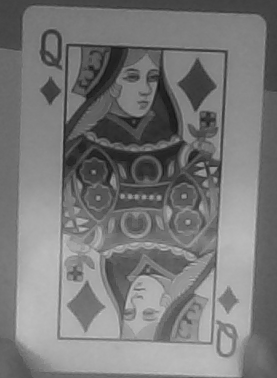
\includegraphics[width=1.3in]{9}
 		\captionof{figure}{Imagem base 1 - carta de baralho. Tirada pela pr\'opria webcam.}
 		\end{minipage}			
 		
 		\vspace{2\baselineskip}\vspace{-\parskip}
 		\begin{minipage}{\linewidth}
 		\centering
 		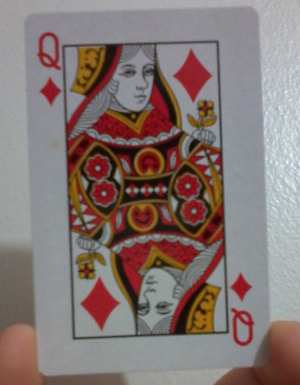
\includegraphics[width=1.3in]{c2}
 		\captionof{figure}{Nova imagem base 1 - carta de baralho. Necess\'ario devido \'a inutiliza\c{c}\~ao de alguns 
 		m\'etodos. Tirada da c\^amera do celular.}
 		\end{minipage}	
 
 		\vspace{2\baselineskip}\vspace{-\parskip}
 		\begin{minipage}{\linewidth}
 		\centering
 		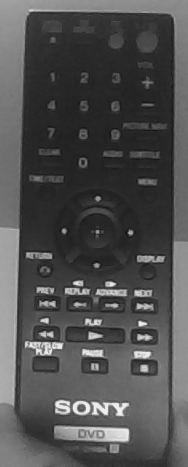
\includegraphics[width=1.3in]{12}
 		\captionof{figure}{Imagem base 2 - controle remoto. Tirada da webcam.}
 		\end{minipage}	
 
		\vspace{2\baselineskip}\vspace{-\parskip}
 		\begin{minipage}{\linewidth}
 		\centering
 		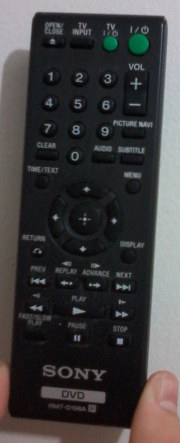
\includegraphics[width=1.3in]{c3}
 		\captionof{figure}{Imagem base 2 - controle remoto. Mesmo motivo da imagem base 1. Tirada da c\^amera do 
 		celular.}
 		\end{minipage}	
 		\vspace{2\baselineskip}\vspace{-\parskip}
 		
 \centering SIFT	\\
 \begin{enumerate}
  \item CARTA
    \begin{itemize}
     \item PERTO (10 cm)
      Da amostra escolhida, SIFT identificou em todas elas. Situa\c{c}\~ao de rota\c{c}\~ao, oclus\~ao, ilumina\c{c}\~ao 
      e inclina\c{c}\~ao tamb\'em foram identificados.
     \item LONGE (30 cm)
      Aqui tamb\'em SIFT mostrou grande efici\^encia e reconheceu todos os casos.
    \end{itemize}
  \item CONTROLE
    \begin{itemize}
     \item PERTO (10 cm)
      Da amostra escolhida, SIFT identificou em 9/10 casos.
     \item LONGE (30 cm)
      Aqui SIFT identificou 8/10 casos. 
    \end{itemize}
 \end{enumerate}

\vspace{1.2\baselineskip}\vspace{-\parskip} 
\raggedright
\nobreak\hspace{.16667em plus .08333em} 
SIFT reconheceu muito bem a maioria dos casos. \'E importante lembrar SIFT n\~ao apresentou problemas com ilumina\c{c}\~ao, 
 o que nos mostra que tem robustez contra ela. Das amostras n\~ao identificadas ambas estavam ligeiramente inclinadas.
 
 		\vspace{2\baselineskip}\vspace{-\parskip}
 		\begin{minipage}{\linewidth}
 		\centering
 		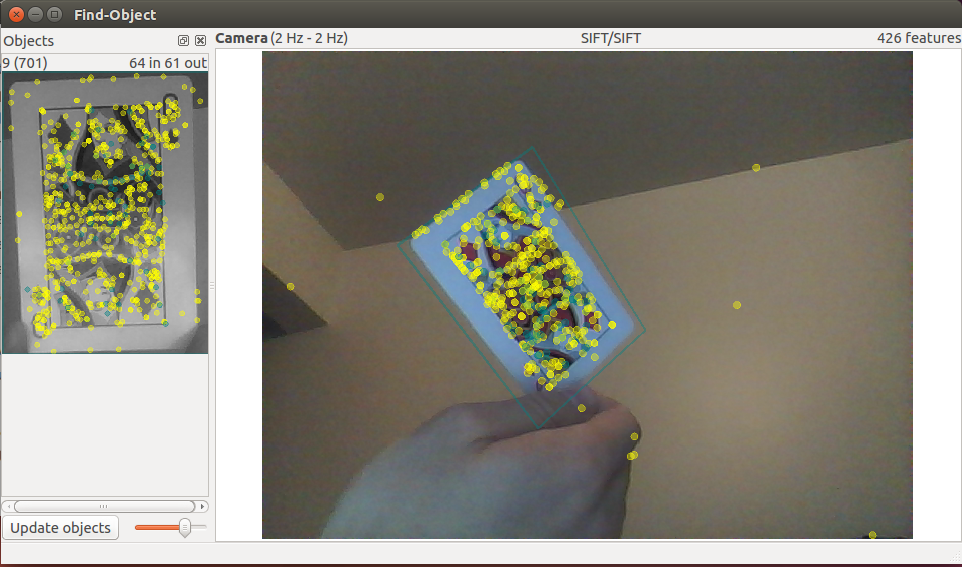
\includegraphics[width=3.3in]{carta8perto}
 		\captionof{figure}{Amostra SIFT carta perto.}
 		\end{minipage}	
 
		\vspace{2\baselineskip}\vspace{-\parskip}
 		\begin{minipage}{\linewidth}
 		\centering
 		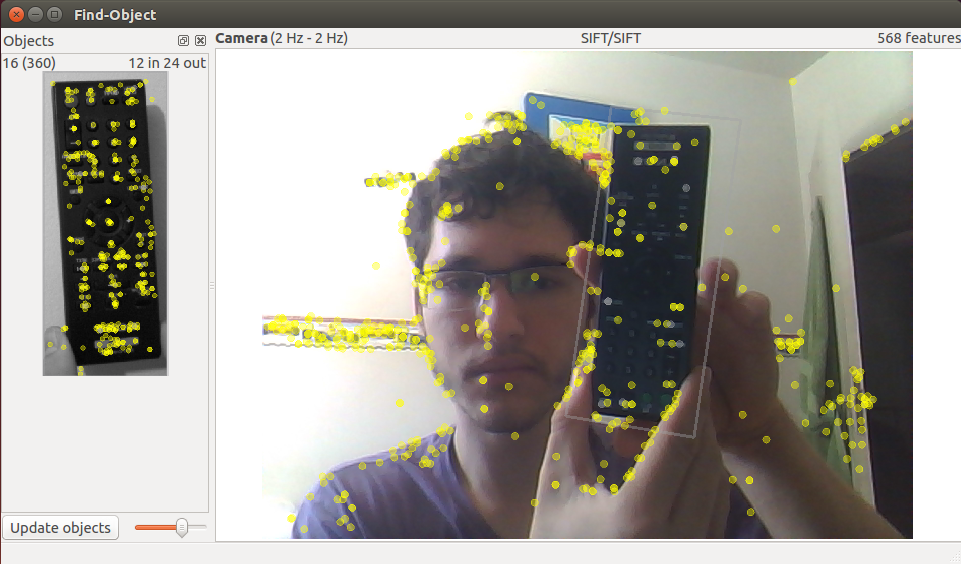
\includegraphics[width=3.3in]{controle10longe}
 		\captionof{figure}{Amostra SIFT controle longe.}
 		\end{minipage}	
 
 
 \vspace{1.2\baselineskip}\vspace{-\parskip} 
 
\centering  SURF
 \begin{enumerate}
  \item CARTA
    \begin{itemize}
     \item PERTO (10 cm)
      SURF encontrou 7/10 amostras. Mostrou-se bom em rela\c{c}\~ao \`a rota\c{c}\~ao. N\~ao foi obtido \^exito em situa\c{c}\~oes 
      onde houve inclina\c{c}\~ao.
     \item LONGE (30 cm)
      \^Exito em 4/10 amostras. SURF n\~ao foi eficiente em rela\c{c}\~ao a dist\^anciamento da c\^amera.
    \end{itemize}
  \item CONTROLE
    \begin{itemize}
     \item PERTO (10 cm)
      Reconheceu 6/10 amostras. Aqui novamente o problema maior foi em rela\c{c}\~ao \`a inclina\c{c}\~ao.
     \item LONGE (30 cm)
      Aqui SURF reconheceu s\'o em um dos casos.
    \end{itemize}
 \end{enumerate}

 \vspace{1.2\baselineskip}\vspace{-\parskip} 
 \raggedright
\nobreak\hspace{.16667em plus .08333em} 
 SURF n\~ao se mostrou eficiente em casos onde houve inclina\c{c}\~ao, dist\^ancia e ilumina\c{c}\~ao. Foi necess\'ario que 
 se utiliza-se a outra imagem base para realizar a compara\c{c}\~ao com as amostras.
 
 		\vspace{2\baselineskip}\vspace{-\parskip}
 		\begin{minipage}{\linewidth}
 		\centering
 		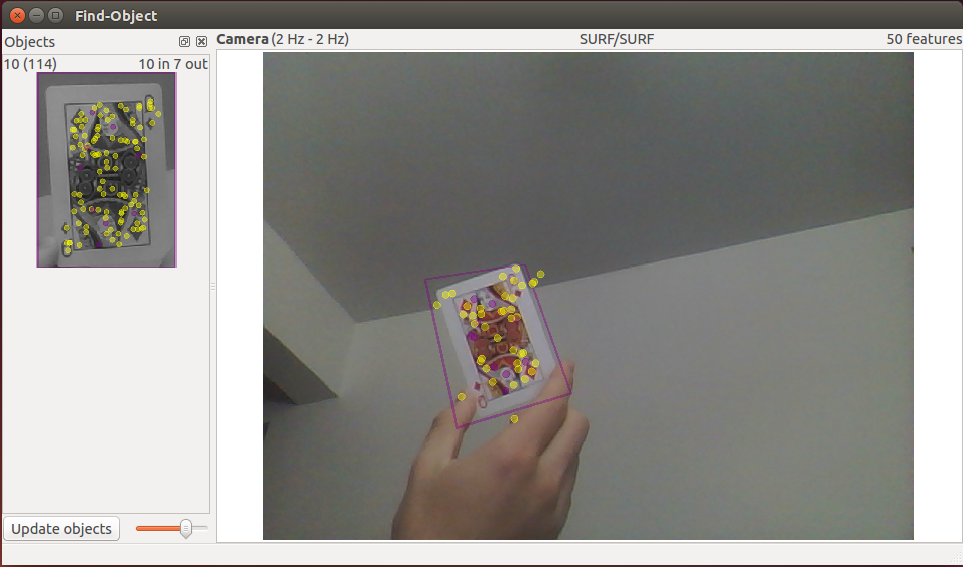
\includegraphics[width=3.3in]{carta5longe}
 		\captionof{figure}{Amostra SURF carta longe.}
 		\end{minipage}	
 
		\vspace{2\baselineskip}\vspace{-\parskip}
 		\begin{minipage}{\linewidth}
 		\centering
 		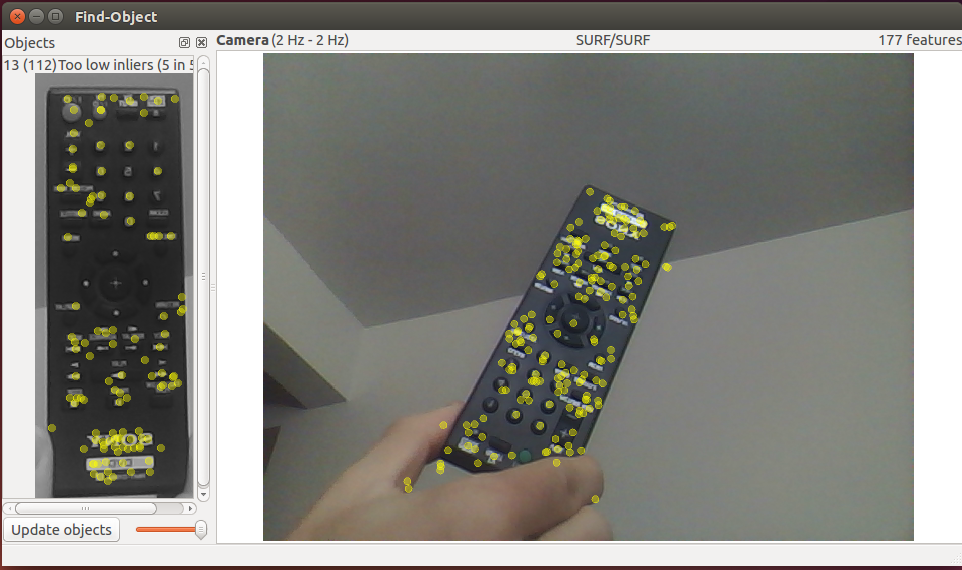
\includegraphics[width=3.3in]{controle6perto}
 		\captionof{figure}{Amostra SURF controle perto.}
 		\end{minipage}	 
 
 
 
 \vspace{1.2\baselineskip}\vspace{-\parskip} 
 
 \centering FAST/BRIEF
  \begin{enumerate}
  \item CARTA
    \begin{itemize}
     \item PERTO (10 cm)
      Encontrou 5/10 casos. Rota\c{c}\~ao e inclina\c{c}\~ao foram praticamente ignorados. N\~ao houve bom reconhecimento 
      nestes casos. Alguns ru\'idos tamb\'em ocorreram.
     \item LONGE (30 cm)
      Reconheceu 2/10 casos. N\~ao se mostrou muito eficiente \'a uma dist\^ancia maior.
    \end{itemize}
  \item CONTROLE
    \begin{itemize}
     \item PERTO (10 cm)
      Encontrou em 5/10 casos. Aqui rota\c{c}\~oes pequenas foram encontradas, por\'em as maiores e inclina\c{c}\~oes foram 
      ignoradas.
     \item LONGE (30 cm)
      Aqui n\~ao reconheceu nenhum caso.
    \end{itemize}
 \end{enumerate}

\vspace{1.2\baselineskip}\vspace{-\parskip} 
\raggedright
\nobreak\hspace{.16667em plus .08333em} 
 FAST/BRIEF n\~ao se mostrou eficiente \`a longas dist\^ancias e a rota\c{c}\~oes e inclina\c{c}\~oes. Al\'em disto, foi-se 
 necess\'ario usar outra imagem base devido \`a ilumina\c{c}\~ao. Desta forma, n\~ao houve efici\^encia contra ilumina\c{c}\~ao.

 		\vspace{2\baselineskip}\vspace{-\parskip}
 		\begin{minipage}{\linewidth}
 		\centering
 		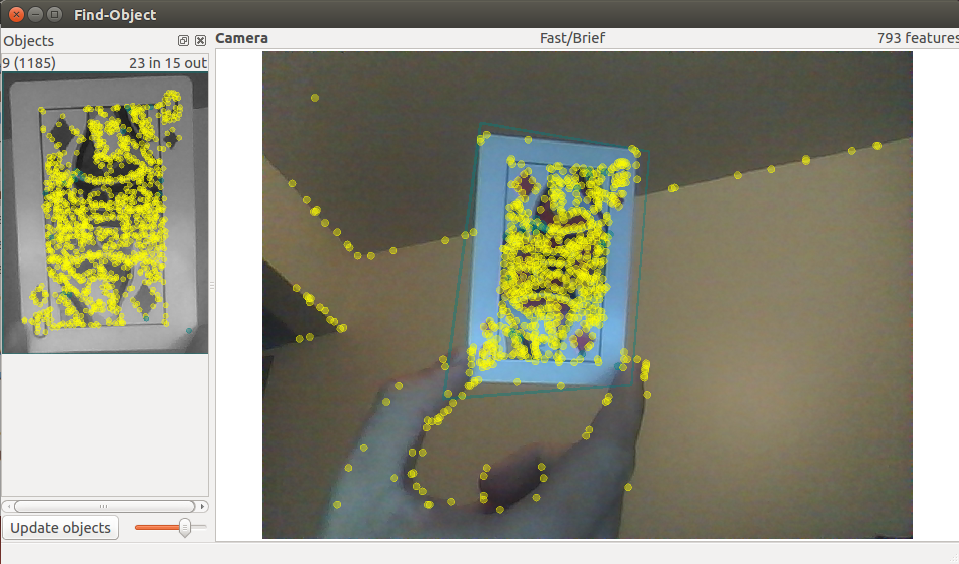
\includegraphics[width=3.3in]{carta1perto}
 		\captionof{figure}{Amostra FAST/BRIEF carta perto.}
 		\end{minipage}	
 
		\vspace{2\baselineskip}\vspace{-\parskip}
 		\begin{minipage}{\linewidth}
 		\centering
 		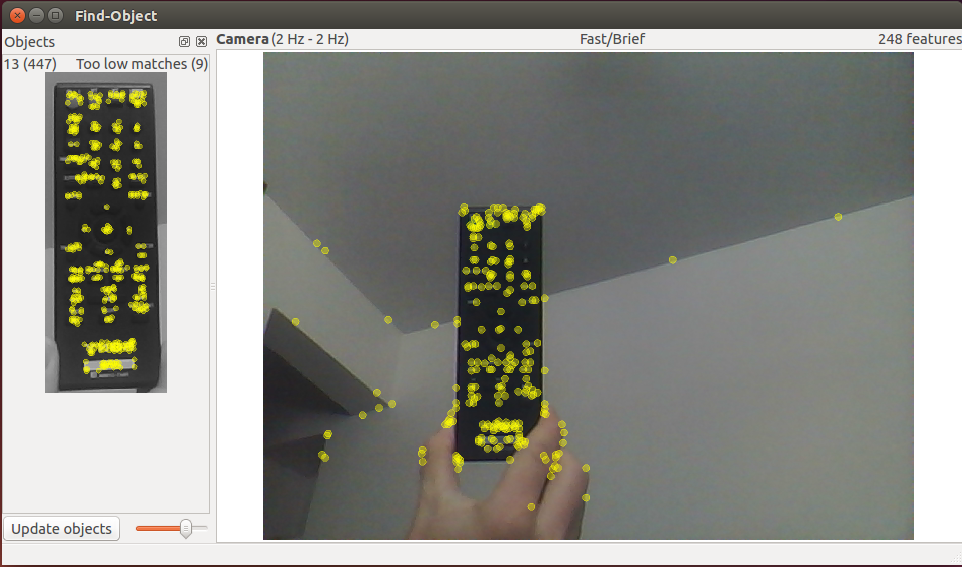
\includegraphics[width=3.3in]{controle1longe}
 		\captionof{figure}{Amostra FAST/BRIEF controle longe.}
 		\end{minipage}	
 
 \vspace{1.2\baselineskip}\vspace{-\parskip} 

\centering  ORB
  \begin{enumerate}
  \item CARTA
    \begin{itemize}
     \item PERTO (10 cm)
      ORB encontrou em 9/10 casos. Assim como o SIFT, mostrou grande efici\^encia em situa\c{c}\~ao de rota\c{c}\~ao, 
      oclus\~ao, ilumina\c{c}\~ao e inclina\c{c}\~ao.
     \item LONGE (30 cm)
      ORB encontrou em todos os casos.
    \end{itemize}
  \item CONTROLE
    \begin{itemize}
     \item PERTO (10 cm)
      ORB reconheceu 9/10 casos. Mostrou-se bem eficiente \`as situa\c{c}\~oes mencionadas acima. O caso n\~ao identificado 
      estava com inclina\c{c}\~ao consider\'vel. Tamb\'em houve ru\'ido em um deles.
     \item LONGE (30 cm)
      ORB reconheceu 6/10. Houve dificuldade para dist\^ancias consider\'aveis. Houve muito ru\'ido tamb\'em naqueles que 
      foram reconhecidos.
    \end{itemize}
 \end{enumerate}
	
\vspace{1.2\baselineskip}\vspace{-\parskip} 
\raggedright
\nobreak\hspace{.16667em plus .08333em} 
 ORB reconheceu grande parte das amostras, tendo nestas condi\c{c}\~oes obtido desempenho similar ao SIFT. Teve alguns problemas 
 apenas na detec\c{c}\~ao do segundo objeto quando este estava mais distante. Em termos de velocidade, pareceu mais r\'apido 
 que o SIFT, sendo este dado estimado por observa\c{c}\~ao do desempenho do computador.

 		\vspace{2\baselineskip}\vspace{-\parskip}
 		\begin{minipage}{\linewidth}
 		\centering
 		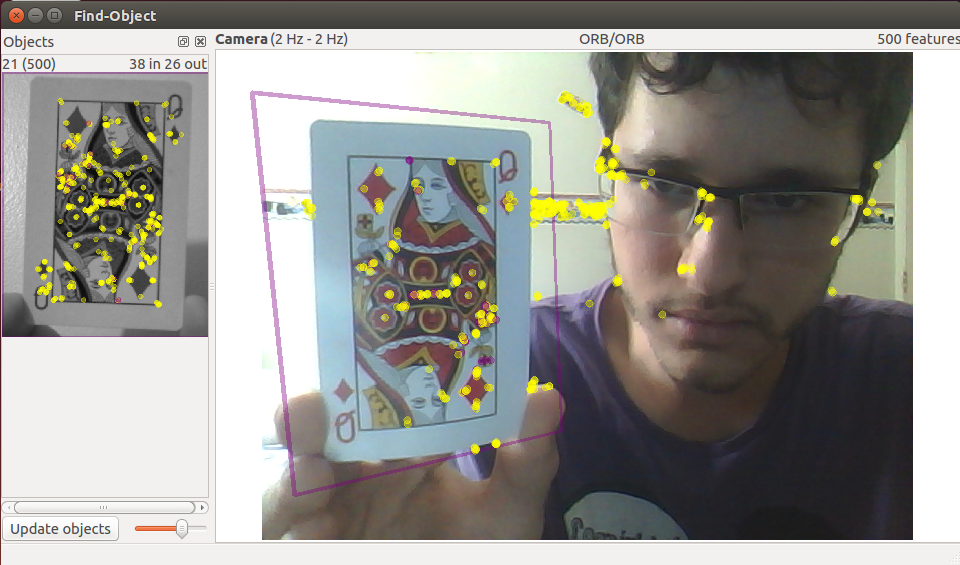
\includegraphics[width=3.3in]{cartaperto5}
 		\captionof{figure}{Amostra ORB carta perto.}
 		\end{minipage}	
 
		\vspace{2\baselineskip}\vspace{-\parskip}
 		\begin{minipage}{\linewidth}
 		\centering
 		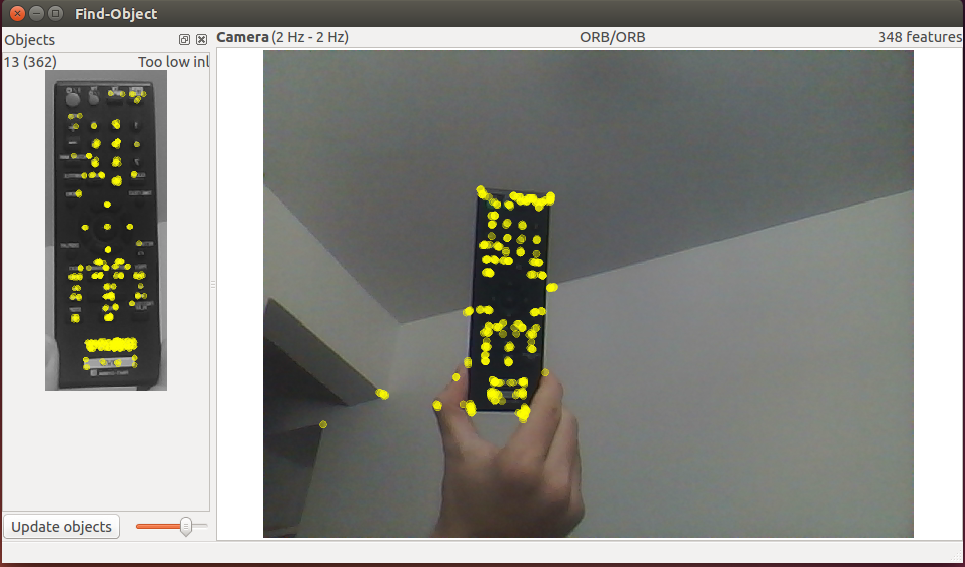
\includegraphics[width=3.3in]{controle3longe}
 		\captionof{figure}{Amostra ORB controle longe.}
 		\end{minipage} 
 
 
 \vspace{1.2\baselineskip}\vspace{-\parskip} 
	
	
\section{Conclus\~ao} 
\label{sec:meth} 

\nobreak\hspace{.16667em plus .08333em} 
Para as situa\c{c}\~oes impostas no proposto experimento, pudemos dizer que SIFT obteve os melhores resultados, seguido de ORB, 
SURF e FAST/BRIEF, sendo que os dois \'ultimos n\~ao obtiveram bons resultados, j\'a que a vari\^ancia \`a ilumina\c{c}\~ao 
esteve presente em ambos. Pudemos notar tamb\'em que o reconhecimente \'e muito dependente do objeto a ser reconhecido.


\section{Refer\^encias} 
\label{sec:meth} 

[1]http://www.mathworks.com/matlabcentral/answers/166657-\\
difference-between-feature-detection-extraction-descriptor-selection-and-matching
    
[2]http://stackoverflow.com/questions/6832933/difference-\\
between-feature-detection-and-descriptor-extraction

[3]https://computervisionblog.wordpress.com/2012/02/10/the-\\
ost-cited-papers-in-computer-vision/

[4]https://www.willowgarage.com/sites/default/files/orb\_\\
final.pdf

[5]http://web.eecs.umich.edu/~silvio/teaching/EECS598/lectu\\
res/lecture10\_1.pdf

[6]http://www.cs.berkeley.edu/~malik/cs294/lowe-ijcv04.pdf

[7]http://www.vision.ee.ethz.ch/~surf/eccv06.pdf

[8]http://homepages.inf.ed.ac.uk/rbf/CVonline/LOCAL\_COPIES\\
/AV1011/AV1FeaturefromAcceleratedSegmentTest.pdf

[9]https://www.robots.ox.ac.uk/~vgg/rg/papers/CalonderLSF10\\
.pdf

[10]http://computer-vision-talks.com/articles/2011-01-04-com\\
parison-of-the-opencv-feature-detection-algorithms/

[11]http://opencv-python-tutroals.readthedocs.org/en/latest/\\
py\_tutorials/py\_feature2d/py\_sift\_intro/py\_sift\_intro.html
     
[12]http://opencv-python-tutroals.readthedocs.org/en/latest/py\\
\_tutorials/py\_feature2d/py\_surf\_intro/py\_surf\_intro.html
     
[13]http://opencv-python-tutroals.readthedocs.org/en/latest/py\\
\_tutorials/py\_feature2d/py\_fast/py\_fast.html

[14]http://opencv-python-tutroals.readthedocs.org/en/latest/py\\
\_tutorials/py\_feature2d/py\_brief/py\_brief.html

\end{document}